\documentclass[pdf]{beamer}
\mode<presentation>{}
\usepackage{minted}
\usepackage{tikz}
\usepackage{pgffor} %% gives looping with \foreach
\usepackage[absolute,overlay]{textpos}
\usepackage{lmodern} %% scalable latin characters
\usetikzlibrary{arrows,shapes,backgrounds}
\usepackage{multirow}
\usepackage{listings} %% another package for code related stuff

%% stuff for minted
\definecolor{mintedBg}{rgb}{0.95, 0.95, 0.95}
\definecolor{blockBg}{rgb}{0.6, 0.6, 0.95}
\definecolor{rnaColor}{rgb}{0, 0.6, 0}
\definecolor{cdsColor}{rgb}{0, 0.4, 0.4}
\definecolor{rnaPol}{rgb}{0.8,0,0.8}
\definecolor{ribosomeCol}{rgb}{0.5,0.5,0.1}
\definecolor{protColor}{rgb}{0.6,0,0.6}
%% colours for nucleotides:
\definecolor{dACol}{rgb}{0.5, 0.5, 0}
\definecolor{dCCol}{rgb}{0.8, 0, 0}
\definecolor{dGCol}{rgb}{0, 0.8, 0}
\definecolor{dTCol}{rgb}{0, 0, 0.8}

\definecolor{navy}{rgb}{0, 0, 0.6}
\definecolor{pur}{rgb}{0, 0, 0.6}
\definecolor{pyr}{rgb}{0.6, 0, 0.2}
%% define styles for different codes
\newminted{cpp}{linenos, bgcolor=mintedBg, fontsize=\footnotesize}
%% then use \begin{cppcode}
\newminted{c}{linenos, bgcolor=mintedBg, fontsize=\footnotesize}
\newminted{perl}{linenos, bgcolor=mintedBg, fontsize=\footnotesize}
\newminted{sh}{linenos, bgcolor=mintedBg, fontsize=\footnotesize,
  language=bash}
\newminted{console}{linenos, bgcolor=mintedBg, fontsize=\footnotesize}

%% a command to define a subheading
\newcommand\subHeading[1]{
  \par\bigskip {\Large\bfseries#1}\par\smallskip
}

%% I detest indentation in footnotes etc, so try this:
\makeatletter
\renewcommand\@makefntext[1]{\noindent\makebox[0em][r]{\@makefnmark}\tiny#1}
\makeatother
%% the makeatletter and makeatother are required to allow me to
%% to change the macro beginning with an @. (though when I call it
%% I don't use the @ ... 

\setlength\parskip{0.5em}
\setlength\parindent{0ex}

%% to have footnotes without references. This from tex.stackexchange.com
\newcommand\blfootnote[1]{%
  \begingroup  %% this makes it a local redefinition
  \renewcommand\thefootnote{}\footnote{#1}%
  \addtocounter{footnote}{-1}  % this adjusts the footnote counter
  \endgroup
}


\title{Scripts and Programs}
\subtitle{Automating simple to complex tasks}
\author{Martin Jakt}

\begin{document}

\begin{frame}
  \titlepage
\end{frame}

\begin{frame}{Program or Script?}
  Both are implemented in some type of computing language.

  No clear dividing line, but usually / often:
  \begin{itemize}
    \item{Scripts}
      \begin{itemize}
      \item simple and specific tasks
      \item often throw-away, used for a single task (eg. mapping a load of
        sequences to a genome)
      \item implemented in an interpreted language (i.e. not compiled)
      \item call external programs to perform the main computation
      \item quick to write, slow to run
      \end{itemize}
  \end{itemize}
  
  \begin{itemize}
    \item{Programs}
      \begin{itemize}
      \item bigger more complex tasks
      \item expected to be used on a frequent basis
      \item compiled to machine code
      \item slow to write, quick to run
      \end{itemize}
  \end{itemize}
  
\end{frame}

\begin{frame}{What is a program}
  \begin{columns}
    \begin{column}{0.5\textwidth}
      \begin{figure}[ht]
        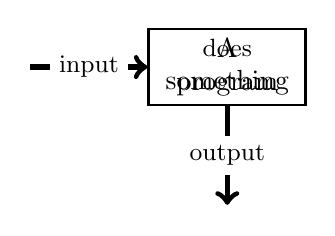
\begin{tikzpicture}[scale=0.5]
          \node [align=center, rectangle, draw=black, line width=1, text=white]
          (b1) at (5,5) {A\\program eh};
          \visible<1-2>{
            \node [align=center, text=black] at (b1) {A\\program}; 
          }
          \visible<2->{
            \draw [->, line width=2] (0,5) -- (b1) node [midway, fill=white]
                  {\small input};
          }
          \visible<3->{
            \draw [->, line width=2] (b1) -- (5,1.5) node [midway, fill=white]
                  {\small output};
            \node [align=center, text=black] at (b1) {\small does\\something}; 
          }
          \end{tikzpicture}
        \end{figure}
    \end{column}
    \begin{column}{0.5\textwidth}
      \visible<4->{
        Need:
        \begin{itemize}
        \item Input data:
          \begin{itemize}
          \item Specified at start of run
          \item Read interactively
          \item From files
          \end{itemize}
        \item Output data:
          \begin{itemize}
          \item Text to screen or file
          \item Binary data to file
          \item Picture (binary data) to screen
          \end{itemize}
        \end{itemize}
      }
    \end{column}
  \end{columns}
\end{frame}

\begin{frame}{Types of interaction}
  In general we can say there are two ways to interact with programs:
  
  \begin{itemize}
    \item Graphical User Interaction (GUI)\\
      Click on pictures and move stuff with a mouse.
      \begin{itemize}
      \item Easy to learn to use
      \item Inflexible
      \item Difficult to automate
      \end{itemize}
    \item Text based Command Line Interfaces (CLI)\\
      Type commands using some sort of defined vocabulary and grammar.
      \begin{itemize}
      \item Harder to learn to use
      \item Flexible
      \item Easy to automate and connect to other programs
      \end{itemize}
  \end{itemize}
  
  \emph{A controlled vocabulary and grammar is the core of any computing
  language. Hence the step from using a CLI to writing scripts / programs is
  rather small.}  
\end{frame}

\begin{frame}[fragile]{The CLI}
  Commands are typed into a terminal or a console.

  \begin{shcode}
    command argument_1 argument_2 argument_3 ...
  \end{shcode}
  
  \begin{itemize}
  \item \texttt{command} is the name of an executable program
  \item \texttt{argument\_n} are the names of arguments to that program; these
    tell the program what to do.
  \end{itemize}
  
  The arguments to the command are the first way to provide input data to the program.
\end{frame}

\begin{frame}[fragile]{Two types of arguments}
  \begin{shcode}
    bowtie -C -f -p 16 --fr ../genomes/index/Gv1_4 seq1.fastq
  \end{shcode}
  
  {\small
  \begin{description}
    \item[options] arguments beginning with \texttt{-} or \texttt{--} are
      (usually) optional and can appear in any order
      \begin{itemize}
      \item standalone (eg. \texttt{-f}) where the simple presence
        of the option is sufficient
      \item with a value specified (eg. \texttt{-p 16} here telling bowtie
        to use 16 threads during the mapping process
      \item \texttt{--} is usually used for long form options (more than a
        single letter)
      \end{itemize}
    \item[standard] arguments are just words seperated by text.
      \begin{itemize}
      \item must be in the correct order
      \item are seperated by spaces; can use \texttt("a stupid filename") to
        specify arguments (eg. filenames) that contain spaces.
      \end{itemize}
  \end{description}
 
  This is true for Unix and MacOS. On Windows options are specifed with the
  forward slash \texttt{"/"}.
  }
\end{frame}

\begin{frame}[fragile]{the PATH environment variable}
  the \texttt{PATH} environment variable contains a set of directories which
  are searched for executable files with names matching the first word of a
  command.

  On Unix based systems you can find out it's value by:
  \begin{shcode}
    echo $PATH
  \end{shcode}
  which on my machine gives:
  
  \texttt{/home/lmj/bin:/usr/local/bin:/usr/bin:/bin:/usr/bin/X11:\\/usr/games:/usr/lib/mit/bin:/usr/lib/mit/sbin}
\end{frame}

\begin{frame}[fragile]{specifying the full path to the program}
  If the program you wish to run is not in any of the directories listed in
  \texttt{\$PATH} you need to specify the location (i.e. the path).

  \begin{shcode}
    ~/apps/bowtie-1.1.2/bowtie -C -f -p 16 --fr \
         ../genomes/index/Gv1_4 seq1.fastq
  \end{shcode}
  
  Here \texttt{\textasciitilde} is shorthand for my home directory, and the program is a version
  of bowtie that I have installed locally (i.e. not requiring root or
  administrator access).

  How to specify file system locations is covered in my previous presentation
  and we will see this in practice further on.
\end{frame}

\begin{frame}[fragile]{the \texttt{./} notation}
  To run a program that is present in the current working directory:

  \begin{shcode}
    ./program_name arg1 arg2 ...
  \end{shcode}

  On Windows I think that the current directory is always part of the PATH,
  but not really sure.
\end{frame}

\begin{frame}[fragile]{reading input}
  Command line programs can read input from:

  \begin{itemize}
  \item \texttt{STDIN} (standard in), either interactively (user types input)
    or through reading the output of programs that print output to
    \texttt{STDOUT}.
  \item Files containing data.
  \end{itemize}

  In general, files containing data and configurations are specified on the
  command line. \texttt{STDIN} and \texttt{STDOUT} are normally used to pass
  output from one program to another.
\end{frame}

\begin{frame}[fragile]{output}
  Output is directed to:
  \begin{itemize}
  \item \texttt{STDOUT}. By default this prints to the terminal, but the
    output can be redirected either to a file or to other processes.
  \item Files.
  \end{itemize}

  Most programming language have some sort of \texttt{print} or \texttt{write}
  function that is used to write data to output.
\end{frame}

\begin{frame}[fragile]{The usual minimal program}
Most introductions to programming languages include a minimal "Hello world"
program, that just prints "Hello world" to the terminal.

In perl:
\begin{perlcode}
#!/usr/bin/perl -w

print "Hello world\n";
\end{perlcode}

To run this program (assuming it is in your current directory):
\begin{consolecode}
lmj:[Perl]> chmod +x helloWorld.pl 
lmj:[Perl]> ./helloWorld.pl 
Hello world
lmj:[Perl]>
\end{consolecode}  
\blfootnote{The details will be explained later}
\end{frame}

\begin{frame}[fragile]{accessing the arguments}
The arguments given to the program are usually available in a data structure
called something like \texttt{argv}. In perl we have an array called
\texttt{@ARGV}. We can modify "helloWorld.pl" to echo it's first argument. In
the file \texttt{echo\_1.pl}:

\begin{perlcode}
#!/usr/bin/perl -w

print "$ARGV[0]\n";
\end{perlcode}

Then to run:
\begin{consolecode}
lmj:[Perl]> chmod +x echo_1.pl 
lmj:[Perl]> ./echo_1.pl Goodbye world
Goodbye
lmj:[Perl]> 
\end{consolecode}

\end{frame}

\begin{frame}{a small console program}
  \begin{enumerate}
  \item inspect the arguments to determine what to do:
    \begin{itemize}
    \item names of files to open
    \item options as to how to process data
    \end{itemize}
  \item open specified files and read data
  \item do something useful with the data
  \item print something useful to terminal (i.e. \texttt{STDOUT}) or to a file
    specified as an argument.
  \end{enumerate}
\end{frame}

\begin{frame}{reading data from a file}
  Data needs to be structured in some manner such that the program can make
  sense of it. For text file usually:
  \begin{itemize}
  \item line delimited (i.e. one line contains one record of data)
  \item individual lines are usually delimited by some special character
    (eg. \texttt{<TAB>}).
  \end{itemize}

  Hence there are many functions for reading one line of text at a time.

  \blfootnote{We will not cover the reading of data from binary files; in
    principle it is no different, but it is not generally delimited by lines,
    but by a more specific structure.}
\end{frame}

\begin{frame}[fragile]{How to process data?}
  Data is processed by something akin to simple algebra. That is we assign the
  values of data elements to variables, and perform operations on
  these. Eg. to add two numbers together in perl:
  
  \begin{perlcode}
    #!/usr/bin/perl -w
    $x = $ARGV[0];
    $y = $ARGV[1];
    $z = $x + $y;
    print "$y\n";
  \end{perlcode}
  
  obviously, this is a stupid example, but at least it's simple.
\end{frame}

\begin{frame}[fragile]{processing data: the toolbox}
  All you need is...

  \begin{itemize}
  \item mathematical functions (eg. arithmetic operators, comparators,
    transformations, etc...)
  \item collections of variables (lists, key-value maps and more complex structures)
  \item conditional statements (eg. if something is true do A, else do B)
  \item loops (e.g. do something to every element of a collection, or until
    some condition is true)
  \item functions to read and write data
  \item custom functions
  \end{itemize}

  to do pretty much anything.
\end{frame}

\begin{frame}[fragile]{variables and collections of variables}
  3 basic groups:
  \begin{description}
  \item[scalar] Each variable holds a single value.
  \item[lists] Each variable points to a list (aka array or vector) of
    values. Individual values are accessed by their position in the list by a
    numerical subscript.
  \item[maps] Variables are stored as key-value pairs. The key can be number
    or a string (i.e. text), or some other type of data and is used to
    access the associated value. In perl a map is called a "hash".
  \end{description}

  You can also combine these to have lists of lists, lists of maps, maps of
  lists.
  \blfootnote{Different languages refer to similar types of collections using
    different names. The ones used here are generic but may have special
    meanings in some languages.}
\end{frame}

\begin{frame}[fragile]{types of data}
  Somewhat simplified:
  \begin{description}
  \item[character] A single byte of data. Usually contains a single ascii
    character (i.e. a roman alpha-numeric character, or a simple control code).
  \item[string] A sequence of characters treated as a single
    variable.
  \item[Numeric values] two main types:
    \begin{description}
    \item[integral values] Signed or unsigned values encoded by 1-8 bytes of
      data per value.
    \item[floating point] Variable precision values usually encoded by 4 or 8
      bytes of data per value.
    \end{description}
  \end{description}
  
  In strongly typed languages you have to specify what the variables
  encode. In dynamically typed languages the interpreter makes a guess and
  tries to do the best with the input it receives.
\end{frame}

\begin{frame}[fragile]{Calculate a gapless alignment score}
  \begin{enumerate}
  \item $m \leftarrow match score$, $mm \leftarrow mismatch penalty$
  \item $s1 \leftarrow first argument$, $s2 \leftarrow second argument$
  \item $score \leftarrow 0$
  \item for each value of $i$ from 1 to length of $s1$:
    \begin{enumerate}
    \item if $s1_i == s2_i$ then \\
      $score \leftarrow score + m$ \\
      else\\
      $score \leftarrow score + mm$
    \end{enumerate}
  \item print $score$
  \end{enumerate}

  Except we count from 0, not 1!\\
  And this won't work if we $s1$ and $s2$ are not the same length.
\end{frame}

\begin{frame}[fragile]{in perl}
  \begin{perlcode}
    #!/usr/bin/perl -w
    $m = 1;
    $mm = -2;
    $score = 0;
    ## This is a comment!
    ## Here, the split command splits a string to
    ## an array (list) where each letter can be
    ## accessed by it's position
    @s1 = split //, $ARGV[0];
    @s2 = split //, $ARGV[1];
    ## for each value from 0 to the
    ## highest index of @s1 assign to $i
    ## and do the stuff inside the braces (curly brackets)
    for $i(0..$#s1){
      if($s1[$i] == $s2[$i]){
        $score = $score + $m;
      }else{
        $score = $score + $mm;
      }
    }
    print "$score\n";
  \end{perlcode}
\end{frame}


\begin{frame}[fragile]{functions (1)}
  These are like mini-programs. A function is a part of a program that can be
  called from anywhere within the program.
  \begin{itemize}
  \item A function is called with a set of arguments.
  \item A function returns a single value; but that value can be a collection
    or more complex data structure containing many individual values.
  \end{itemize}
  
  A function is typically called by its name, with the arguments following
  enclosed in brackets and seperated by commas:


  \begin{cppcode}
    var1 = function1( arg1, arg2, arg3 )
  \end{cppcode}

  Here the value returned by \texttt{function1} is assigned to the variable
  \texttt{var1}. 

\end{frame}

\begin{frame}[fragile]{functions (2)}
  In addition to returning a value, a function can have side-effects:

  \begin{itemize}
  \item It may be able to modify the values of its arguments\footnote{This
    depends on the language used and how the function is defined.}
  \item Print stuff to the screen, including displaying graphics.
  \item Write data to files.
  \item Control peripherals (a superset of displaying stuff).
  \end{itemize}
  
  There is a school of programming that considers side effects to be evil; but
  a program without side effects can not be useful!
\end{frame}

\begin{frame}[fragile]{functions (3)}
  \begin{description}
  \item[built-in] Most (all?) programming languages come with a set of built
    in functions which are always available to the programmer. In general the
    higher level the language the more the functions.
  \item[library] In general you can also import functions from libraries of
    functions. This is done differently depending on the language, but once
    imported they can be used as normal functions.
  \item[user generated] These are usually written as part of most
    programs. They generalise operations that are performed repeatedly within
    the program and decrease the amount of code that needs to be written.
  \end{description}
\end{frame}

\begin{frame}[fragile]{data structures}
  Organising data into a reasonable structure is essential to any more
  complicated program.

  But, erhm, sorry I'm ignoring this for the time being as we will restrict ourselves to
  simple things in perl, which isn't really good for complex data
  structures. Anyway, you'll be exposed to some horrible perl data structures
  presently...

\end{frame}

\begin{frame}[fragile]{mathematical operators (1)}
  Operators are like special types of functions that make use of normal
  symbols for mathematical operations:

  Calling a function to add two numbers:
  \begin{cppcode}
    a = sum(b, c);
  \end{cppcode}

  Instead we can write:
  \begin{cppcode}
    a = b + c;
  \end{cppcode}

  The set of operators vary a little bit between languages, but most normal
  arithmetic operations are usually included.

\end{frame}

\begin{frame}[fragile]{mathematical operators (2)}
  \footnotesize{
  \begin{description}
    \item[+, -, /, *] return the expected value ($a + b$) returns the sum of $a$
      and $b$
    \item[\textless, \textgreater, \textless=, \textgreater=] less than, greater than, less than or equal, greater than
      or equal. These return \texttt{TRUE} or \texttt{FALSE} values as
      appropriate.
    \item[==, !=] equality and inequlity operators. Return \texttt{TRUE} and
      \texttt{FALSE} respectively if the values of its
      operands are equal.
    \item[++, --] auto increment and decrement. These increase or decrease the
      value of it's single operand by 1. eg. \texttt{i++;} will increase the
      value of \texttt{i} by 1.
    \item[+=, -=, *=, /=] increase or decrease the value of its first operand by
      the value or multiple of it's second operand. eg. \texttt{a *= b} will
      assign the value of \texttt{a * b} to \texttt{a}.
    \item[\%] the modulus operator; returns the remainder of an implied
      division. eg. \texttt{10 \% 3} will return a value of 1.
  \end{description}
  
  There are some difference between languages, but these can be found in most
  computing languages.
  }
\end{frame}


\begin{frame}[fragile]{scope (1)}
  \begin{itemize}
  \item Variables can be defined locally or globally.
  \item Local variables are only accessible within their scope.
  \end{itemize}

  What does this mean?
\end{frame}


\begin{frame}[fragile]{scope (2)}
  An example in C++:
  \begin{cppcode}
    int sum(int a, int b){
      return(a + b);
    }

    int main(int argc, char **argv){
      int a = 10;
      int b = 10;
      {
        int b = 20;
        a = a + b;
      }
      cout << "sum of 40 and 50 : " << sum(40, 50) << endl;
      cout << "a is : " << a << endl;
      cout << "b is : " << b << endl;
    }
  \end{cppcode}

  This will output ?
\end{frame}

\begin{frame}[fragile]{scope (3)}
  \begin{cppcode}
    cout << "sum of 40 and 50 : " << sum(40, 50) << endl;
    cout << "a is : " << a << endl;
    cout << "b is : " << b << endl;    
  \end{cppcode}
  
  \begin{figure}[ht]
    
\begin{tikzpicture}[scale=1]
      \node [scale=2] at (0,0) {$\Downarrow$};
    \end{tikzpicture}
  \end{figure}

  \begin{consolecode}
    lmj:[cpp]> g++ -o test test.cpp
    lmj:[cpp]> ./test
    sum of 40 and 50 : 90
    a is : 30
    b is : 10
  \end{consolecode}
\end{frame}

\begin{frame}[fragile]{scope (4)}
  \begin{cppcode}
    int sum(int a, int b){
      return(a + b);
    }
  \end{cppcode}
  \small{
  This is in a seperate function. \texttt{a} and \texttt{b} are defined
  locally here, but they have no effect outside of the function.
  }

  \vspace{1em}

  \begin{cppcode}
    {
      int b = 20;
      a = a + b;
    }
  \end{cppcode}
  \small{Here the curly brackets indicate the creation of a new sub-scope. In the sub-scope
  we can access and modify variables defined in the parent
  scope, but variables defined (\texttt{int b = 20}) within the sub-scope can
  not be accessed nor affect variables outside of the sub-scope.
  }
\end{frame}

\begin{frame}{scope (5)}
  \begin{itemize}
  \item Scoping rules vary extensively across programming languages.
  \item For short scripts a global scope is usually OK (as you can easily
    remember all variables and their names).
  \item For longer scripts / programs, rigorously defined scopes are essential
    to not introducing a big pile of bugs.
  \item perl is globally scoped by default. This is convenient to start with,
    but usually comes back and bites you as the complexity of your program
    grows.
  \end{itemize}
\end{frame}

\begin{frame}[fragile]{indentation}
  \begin{perlcode}
    ## for each value from 0 to the
    ## highest index of @s1 assign to $i
    ## and do the stuff inside the braces (curly brackets)
    for $i(0..$#s1){
      if($s1[$i] == $s2[$i]){
        $score = $score + $m;
      }else{
        $score = $score + $mm;
      }
    }
    print "$score\n";
  \end{perlcode}
  \small{Some parts of the code are indented. This is to make it easier to read the
  code. In general there are no specific rules for how to indent, but many
  editors will automatically indent the code. (This really helps to find
  mistakes.)

  In Python, the rules of indentation are part of the language definition, and
  must be followed, as indentation has syntactic meaning.
}
\end{frame}


\begin{frame}{to write a program}
  \begin{enumerate}
  \item Consider how you wish to represent the input data inside of the
    program; eg. as strings, or arrays of characters, as maps or lists.
  \item Decide how to output the data; i.e. define or choose a specific file format.
  \item Identify tasks that are likely to be carried out repetitively within
    the program, and write functions for these.
  \item Write the main body of the program; if the program is well structured,
    this can be rather short.
  \end{enumerate}
\end{frame}

\begin{frame}{shell scripting}
  From the command line to small programs.

  \begin{enumerate}
  \item Combine several commands into a file and get the shell to run the
    commands.
  \item Pipe (pass) output from one program to another.
  \item Add a syntax for performing conditional tests, looping and lists of
    values.
  \end{enumerate}

  Generally text based.
\end{frame}

\begin{frame}[fragile]{shell scripting example (1)}
  Combine the following commands to find and filter (by name) a set of files
  and finally to run a specific command on them.
  
  \begin{description}
  \item[find] searches the file system for files with specific properties
    (including name, and others)
  \item[grep] searches text for matches to text patterns; prints matching
    lines
  \item[read] reads the lines of a file or STDIN assigning the line to a
    variable
  \end{description}

  These are just normal programs that print their output to STDOUT.
\end{frame}


\begin{frame}[fragile]{shell scripting example (2)}
  \begin{shcode}
    ## this searches the specified directory for files ending 
    ## in F3.csfasta
    find ~/genomes/cod/KildinCod/csfasta -name "*F3.csfasta"

    ## This reads lines of text from STDIN and prints those 
    ## that do not contain the string "rejects" to STDOUT
    grep -v rejects

    ## we can combine the two using a "|" symbol (a pipe)
    
    find ~/genomes/cod/KildinCod/csfasta -name "*F3.csfasta" | \
    grep -v rejects

    ## this will print out only those that match both criteria 
    ## to STDOUT. These are the file names that we wish to do 
    ## something to.
    
    ## The \ at the end of the line merely escapes the special 
    ## meaning of a newline and allows me to write the command 
    ## over several lines of text.
  \end{shcode}

\end{frame}

\begin{frame}[fragile]{shell scripting example (3)}
  \small{In order to specify the full
  command line we use while and read to loop through the entries.}

  \begin{shcode}
    find ~/genomes/cod/KildinCod/csfasta -name "*F3.csfasta"|\
          grep -v rejects|while read fname; do
          ## use other programs to format some filenames
          fb=`basename -s F3.csfasta $fname`
          sam=$samDir$(basename -s _ $fb)".sam"
          
          bowtie -C -f -p 16 --fr ~/bwt_index/Gv1 $fname $sam
    done
  \end{shcode}

  \small{this example much simplified to fit in the presentation.}

\end{frame}

\begin{frame}{shell scripting}
  Very convenient.

  But to be honest, I really don't like the syntax much.
\end{frame}

\end{document}
